\documentclass[12pt,a4paper]{article}

%%%%%%%%%%%%%%%%%%%%%%%%% packages %%%%%%%%%%%%%%%%%%%%%%%%
\usepackage{tikz}
\usepackage{verbatim}
\usepackage{graphicx}
\usepackage{subcaption}
\usetikzlibrary{arrows,shapes}
\usepackage{amsmath}
\usepackage{amssymb}
\usepackage{physics}
\usepackage{amsthm}
\usepackage{amsmath}
\usepackage{amsfonts}
\usepackage{graphicx}
\usepackage[all]{xy}
\usepackage{tikz}
\usepackage{verbatim}
\usepackage[left=2cm,right=2cm,top=3cm,bottom=2.5cm]{geometry}
\usepackage{hyperref}
\usepackage{caption}
\usepackage{subcaption}
\usepackage{psfrag}

%%%%%%%%%%%%%%%%%%%%% students data %%%%%%%%%%%%%%%%%%%%%%%%
\newcommand{\student}{Your full name here!}
\newcommand{\course}{Course name goes here!}
\newcommand{\assignment}{Put a number here!}

%%%%%%%%%%%%%%%%%%% using theorem style %%%%%%%%%%%%%%%%%%%%

\newtheorem{thm}{Theorem}
\newtheorem{lem}[thm]{Lemma}
\newtheorem{defn}[thm]{Definition}
\newtheorem{exa}[thm]{Example}
\newtheorem{rem}[thm]{Remark}
\usepackage{braket}
\newtheorem{coro}[thm]{Corollary}
\newtheorem{quest}{Question}[section]

%%%%%%%%%%%%%%  Shortcut for usual set of numbers  %%%%%%%%%%%

\newcommand{\N}{\mathbb{N}}
\newcommand{\Z}{\mathbb{Z}}
\newcommand{\Q}{\mathbb{Q}}
\newcommand{\R}{\mathbb{R}}
\newcommand{\C}{\mathbb{C}}
\newcommand{\tens}[1]{%
	\mathbin{\mathop{\otimes}\limits_{#1}}%
}

%%%%%%%%%%%%%%%%%%%%%%%%%%%%%%%%%%%%%%%%%%%%%%%%%%%%%%%555
\begin{document}
\pgfdeclarelayer{background}
\pgfsetlayers{background,main}


%%%%%%%%%%%%%%%%%%%%%%% title page %%%%%%%%%%%%%%%%%%%%%%%%%%
\thispagestyle{empty}
\begin{center}
\textbf{AFRICAN INSTITUTE FOR MATHEMATICAL SCIENCES \\[0.5cm]
(AIMS RWANDA, KIGALI)}
\vspace{1.0cm}
\end{center}

%%%%%%%%%%%%%%%%%%%%% assignment information %%%%%%%%%%%%%%%%
\noindent
\rule{17cm}{0.2cm}\\[0.3cm]
Name: Sittana Osman Afifi Mohamedelmubarak \hfill  ch 2\\[0.1cm]
Zero-Knowledge proofs: Implementation of the Graph Isomorphism Protocol  \hfill Date: \today\\
\rule{17cm}{0.05cm}
\vspace{1.0cm}

\section{Graph isomorphism}
\begin{defn}(Graph)\cite{gross2003handbook:5}:A graph consist of set of vertices(nodes) $V$ and set of edges $E$.\\
Two nodes $u$ and $v$ is said to be adjacent if there is an edge $(u,v) \in E$.
\end{defn}
we can describe graph using adjacency matrix which is a square matrix $M_{n\times n}$, with $[m_{ij}]=1 $ if $(i,j)\in E$ and $0$ otherwise.     
\begin{defn}
Let $V(G)$, $E(G)$ denote the vertex set and edge set of $G$ respectively. Then, a pair of of graphs$(G_0, G_1)$is \textbf{isomorphic} (denoted $G_0\simeq G_1$) if there exists a permutation $\Pi:V(G0)\longmapsto V(G1)$such that $\forall x,y \in V(G_0), xy\in E(G_0)$ if and only if $\Pi(x)\Pi(y)\in E(G_1)$. The permutation $\Pi$ is called an isomorphism.\cite{lec-notes1:3}
\end{defn}
In other words: two graphs are said to be isomorphic if after we relabeling vertices in one graph we get the other graph (the same adjacency matrix).
\begin{exa}
 Two isomorphic graphs with their corresponding adjacency matrices.
\begin{figure}[h!]
	\centering
	\begin{subfigure}[b]{.29\linewidth}
		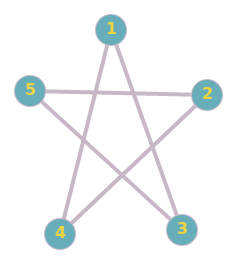
\includegraphics[width=\linewidth]{ex1_1.png}
		\caption{$G_0$.}
	\end{subfigure}
	\begin{subfigure}[b]{.24\linewidth}
		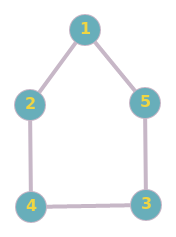
\includegraphics[width=\linewidth]{ex1_2.png}
		\caption{$G_1$.}
	\end{subfigure}
	\caption{Two isomorphic graphs.}
	\label{fig:Two isomorphic graphs}
\end{figure}
\begin{table}[!htb]
	%\caption{Crossponding ajacency matrix }
	\begin{minipage}{.5\linewidth}
		
		\centering
		\begin{tabular}{|c|c|c|c|c|c|}
			\hline 
			& \textbf{1} & \textbf{2} & \textbf{3} & \textbf{4} & \textbf{5} \\ 
			\hline 
			\textbf{1} & 0 & 0 & 1 & 1 & 0 \\ 
			\hline 
			\textbf{2} & 0 & 0 & 0 & 1 & 1 \\ 
			\hline 
			\textbf{3} & 1 & 0 & 0 & 0 & 1 \\ 
			\hline 
			\textbf{4} & 1 & 1 & 0 & 0 & 0 \\ 
			\hline 
			\textbf{5} & 0 & 1 & 1 & 0 & 0 \\ 
			\hline  
		\end{tabular} 
	\caption{ajacency matrix of $G_0$}
	\end{minipage}%
	\begin{minipage}{.5\linewidth}
		\centering

		\begin{tabular}{|c|c|c|c|c|c|}
			\hline 
			& \textbf{1} & \textbf{2} & \textbf{3} & \textbf{4} & \textbf{5} \\ 
			\hline 
			\textbf{1} & 0 & 1 & 0 & 0 & 1 \\ 
			\hline 
			\textbf{2} & 1 & 0 & 0 & 1 & 0 \\ 
			\hline 
			\textbf{3} & 0 & 0 & 0 & 1 & 1 \\ 
			\hline 
			\textbf{4} & 0 & 1 & 1 & 0 & 0 \\ 
			\hline 
			\textbf{5} & 1 & 0 & 1 & 0 & 0 \\ 
			\hline 
		\end{tabular}
			\caption{ajacency matrix of $G_1$}
	\end{minipage} 
\end{table}

Graph (b) is obtained, by relabeling the vertices of Graph (a) according to the following permutation: (1, 4, 5, 2, 3). This means that Node 3 in Graph (a) becomes Node 5 in Graph (b), Node 4 becomes Node 2. 
\end{exa}
\subsection{Graph Isomorphism based Zero-Knowledge Proofs}
Suppose we have two isomorphic graphs $G_0$ and $G_1$ and $G_1=\Pi(G_0)$, with limited messages between the prover and verifier, $P$ wants to prove to $V$ he knows the secret $\Pi$ without showing him what is $\Pi$ exactly.
From the previous example, we can see that it is easy to show that two graphs are isomorphic or not but this process isn’t always simple; suppose we have two graphs have $10$ vertices and $28$ edges, like these graphs:
\begin{figure}[h!]
	\centering
	\begin{subfigure}[b]{.39\linewidth}
		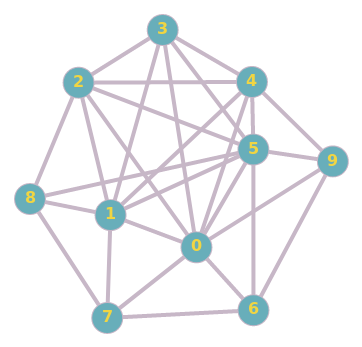
\includegraphics[width=\linewidth]{ex2_1.png}
		\caption{$G_0$.}
	\end{subfigure}
	\begin{subfigure}[b]{.39\linewidth}
		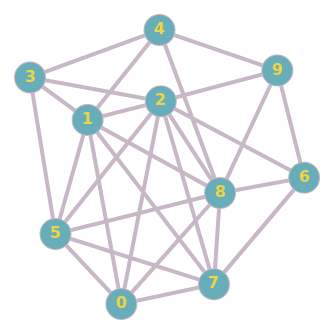
\includegraphics[width=\linewidth]{ex2_2.png}
		\caption{$G_1$.}
	\end{subfigure}
	\caption{Two isomorphic graphs.}
	\label{fig:Two isomorphic graphs has 10 vertices and 28 edges}
\end{figure}\\
So ZKP can provide a protocol that the $P$ can prove to $V$ he knows the secret $\Pi$ without revealing $\Pi$ itself.\\
The protocol is done by apply random permutation ($\varphi$) on $G_0$, with: $$H=\varphi(G_0)$$ and the honest prover has to be able to find a permutation such that he could transform $H$ to either $G_0$ or $G_1$.(i.e to prove $H\simeq G_0$ or $H\simeq G_1$)\\
\subsection{ Zero-Knowledge Protocol for Graph Isomorphism}
We have two graphs known by both parties $G_0$ and $G_1$ such that they have $n$ vertices, define $s_n$ as a set of permutations has $n$ element.\\   
The protocol proceeds by the following:\cite{lec-notes1:3}\\
\textbf{Input}: pair of graphs $(G_0,G_1)$
\begin{enumerate}	
	\item
	\begin{enumerate}
\textbf{prover} chooses random permutation $\sigma$ from $s_n$, and apply $H=\sigma(G_0)$.
\end{enumerate}
	\item
\begin{enumerate}
\textbf{verifier}  chooses $ch$ randomly from $\{0,1\}$ and send it to the prover.
\end{enumerate}
	\item
\begin{enumerate}
\textbf{prover} if $ch=0$: $\varphi=\sigma$ else $\varphi=\sigma \circ \Pi^{-1}$.
\end{enumerate}
	\item
\begin{enumerate}
\textbf{verifier} output \underline{ACCEPT} iff $H=\varphi(G_{ch})$ else output is \underline{REJECT}.\\

\end{enumerate}
\end{enumerate}

\begin{thm}\cite{lec-notes1:3}
The above protocol satisfies completeness, soundness $\frac{1}{2}$, and zero-knowledge.	
\end{thm}
\textbf{Proof}\\
\textbf{Completeness.}
In order to show this protocol is complete, we have to show that if the prover knows the correct permutation $\Pi$ and interacts with an honest verifier, the output will be \textbf{ACCEPT}.\\
Assume we have two isomorphic graphs with a witness $\Pi$ such that $G_1=\Pi(G_0)$, we will check when $ch=0$ an $ch=1$:\\
\begin{enumerate}	
\item
\begin{enumerate}
case 1 ($ch=0$): $P$ has to find a map from $H$ to $G_0$, or to show that $H\simeq \varphi(G_0)$:\\
Since $H=\sigma(G_0)$ then the prover will return $\varphi = \sigma $.Certainly $\sigma(G_0)\simeq \sigma(G_0) $
\end{enumerate}
	\item
	\begin{enumerate}
case 2 ($ch=1$): $P$ has to find a map from $H$ to $G_1$ or to show that $H\simeq \varphi(G_1)$:
		We know that: $$G_1=\Pi(G_0)$$ and $$H=\varphi(G0)$$ then:\\
		$$H=\varphi(\Pi^{-1}(G_1)$$
		$$H=(\varphi \circ 
		\Pi^{-1})(G_1)$$
		So the $$\varphi=\varphi \circ \Pi^{-1}$$
because $$\varphi(G_1)=\sigma \circ \Pi^{-1}(G_1)=\sigma(G0)=H$$
	\end{enumerate}
\end{enumerate}
\textbf{Soundness $\frac{1}{2}$.}
if $G_0\nsim G_1$ then for every probabilistic polynomial time algorithm algorithm $\hat{P}$, there exist a negligible function $negl(\cdot)$ such that:\\
$$Pr[\hat{P}\text{ convinces} V \text{that }G0\simeq G1]\leq negl(\cdot)$$
but $negl(\cdot)=\frac{1}{2}$ because:\\
suppose $G_0\nsim G_1$, since $\simeq$ is transitive so for any graph ${G}^{'}$either ${G}^{'}\simeq G_0$ or ${G}^{'}\simeq G_1$ not both; this indicate that the prover could pass only one of the tests not both.\\
In other words, the prover will pass the test when the verifier choose $ch=0$ because he will return $\sigma$, but he could not pass the test when the verifier choose $ch=1$ because the prover can not find $\varphi$ with $\sigma(G_0)\simeq \varphi(G_1)$ since $G_0\nsim G_1$.\\
since the verifier has only two possible choices $\{0,1\}$ then:
$$Pr[\hat{P}\text{ convinces} V \text{that }G0\simeq G1]\leq \frac{1}{2}$$
\textbf{zero-knowledge.}
Our goal is to construct a simulator S which produces a transcript that is computationally indistinguishable from the execution of the above protocol between an honest prove and an honest verifier.
\textit{suggested protocol}::Define $S$ as follow,\\
\begin{enumerate}	
	\item
	\begin{enumerate}
Sample $\sigma \longleftarrow S_n$ and choose $b \longleftarrow {0,1}$, put $H=\sigma(G_b)$.
\end{enumerate}
\item
\begin{enumerate}
Choose $ch \longleftarrow \{0,1\}$.
\end{enumerate}
\item
\begin{enumerate}
If $ch=b$ output $\sigma$,otherwise repeat from (1).
\end{enumerate}
\item
\begin{enumerate}
Output \textbf{ACCEPT}.
\end{enumerate}
\end{enumerate}
The simulator should protect the honest prover from a cheating verifier who wants to learn more about the secret from the verifier,  but according to the suggested protocol above a cheating verifier can be unfair on how will choose $ch$, $V$ may decide to always send $ch=1$ then $V$ will always send $ch=1$ whereas the simulator $S$ will set $ch=1$ always with probability $\frac{1}{2}$. since $S$ will be always fair and the original protocol is unfair the transcript $\tau^{`} \simeq  \tau$ such that $\tau^{`}$ from $S$ and $\tau$ from the original protocol.\\
In order to fix this issue, we can give $S$ access to an arbitrary black-box verifier $V^*$ that provides $S$ with the random bit for $ch$, using $V^*$ we correct the suggested protocol.\\

\textbf{Correct protocol}:Define $S$ as follow,
\begin{enumerate}	
	\item
	\begin{enumerate}
		Sample $\sigma \longleftarrow S_n$ and choose $b \longleftarrow {0,1}$, put $H=\sigma(G_b)$.
	\end{enumerate}
	\item
	\begin{enumerate}
		Feed $H$ into $V^*$ to get $ch$.
	\end{enumerate}
	\item
	\begin{enumerate}
		If $ch=b$ output $\sigma$,otherwise repeat from (1).
	\end{enumerate}
	\item
	\begin{enumerate}
		Output \textbf{ACCEPT}.
	\end{enumerate}
\end{enumerate}
Now, there is no bias with choosing $ch$, the next step is to prove that $\tau \simeq \tau^{'}$, it suffices to show that the distribution of the output from step (1) is indistinguishable from the output of step (1) in the original protocol, since the rest steps are similar when $G_0 \simeq G_1$.\\

\textbf{Fact 1}: \textit{If $G_0\simeq G_1$ then for $\sigma \longleftarrow S_n,$ the distributions${\sigma(G_0)}$ and ${\sigma(G_1)}$ are equal}.\\
\\
Using fact 1 and by the assumption $G_0\simeq G_1$ then we can conclude that ${\sigma(G0)} = {\sigma(G1)}$ for any $\sigma$ is choosen from $S_n$.
On the other hand, when $\sigma \longleftarrow S_n$, a fixed $\sigma^{`}\in S_n$ so $\sigma \circ \sigma^{`}$ still behaves as a uniformly random permutation, Thereafter,\\
$${\sigma(G_0)}={(\sigma \circ \Pi^{-1}(G_1)}={\sigma_{s}(G_b)}$$
When $\sigma_{S}$ is a permutation choose in step (1) of $S$, and $b\longleftarrow\{0,1\}.$
Thus,  the distribution of the output from step (1) and the output of step (1) in the original protocol are the same, so certainly $\tau \simeq_{c} \tau^{'}$.this complete the proof.\\

The verifier to be convinced that the prover is honest($G_0 \simeq G_1 $and he knows $\Pi$) he needs to apply this procedure several times. if we just apply the procedure once the prover may be lucky when the prover chooses $ch=0$  so the probability is $0.5$.\\
but after repeating the procedure $k$ times the probability for the cheating prover to fail is at least $1-\frac{1}{2^{k}}$ according to \textbf{lemma 1} in  \cite{lec-notes2:6}, if we put $k=10$ the probability would be at least $99.90\%$.\\



 
\bibliography{refer}
\bibliographystyle{ieeetr} 
\end{document}